\chapter{Architecture 3 tiers}

\section{Architecture 3 tiers}

\textbf{Mon architecture 3 tiers :} 
s'appuie sur la pile \textbf{Elixir/Phoenix} pour :
\begin{itemize}
    \item Des applications web \textbf{modernes et performantes}.
    \item Une gestion optimisée du \textbf{temps réel} et de la \textbf{concurence}.
\end{itemize}

\subsection{Couche Présentation (Frontend)}

\begin{for_you}{Technologies de présentation et Structure des composants :}
    \textbf{Technologies de présentation :}
    \begin{itemize}
        \item \textbf{Framework} : Phoenix 1.8.0 + \textbf{LiveView} 1.1
        \item \textbf{Gestion d'état} : GenServer, Agents, ETS (Erlang Term Storage)
        \item \textbf{Base de données} : Ecto (ORM pour PostgreSQL)
        \item \textbf{Routing} : Pipeline Plug (middleware HTTP)
        \newline
    \end{itemize}

    \textbf{Structure des composants :}
    \begin{verbatim}
    badge_reader/
    +-- _build/                            #Compile directory
    +-- assets/
    +-- config/
    +-- deps/
    +-- lib/                               #Code directory
    |   +-- badge_reader/                  #Backend directory
    |   +-- badge_reader_web/              #Frontend directory
    |   +-- badge_reader_web.ex
    |   +-- badge_reader.ex
    +-- priv/
    +-- test/                              #Test directory
    +-- .formatter.exs
    +-- AGENTS.md
    +-- mix.exs
    +-- mix.lock                     
    \end{verbatim}
\end{for_you}

\subsection{Couche Logique Métier (Backend)}

\textbf{Couche logique métier :\newline} 
\begin{for_you}{Environnement Mix et organisation du code}
    \textbf{Mix} (outil de build intégré à Elixir) gère :
    \begin{itemize}
        \item La \textbf{compilation} du code.
        \item Les \textbf{dépendances} (comme `npm` pour Node.js ou `Maven` pour Java).
        \item L'\textbf{organisation} du projet :
              \begin{itemize}
                  \item \texttt{lib/} : Code source (backend + frontend).
                  \item \texttt{test/} : Tests unitaires et d'intégration.
              \end{itemize}
    \end{itemize}
\end{for_you}

\subsubsection{Controller}

\begin{for_you}{Exemple de contrôleur Phoenix}
    \begin{lstlisting}
    # Dans le dossier lib/badge_reader_web/controllers/badge_reader_controller.ex

    defmodule BadgeReaderWeb.BadgeReaderController do
        use BadgeReaderWeb, :controller

        def home_page(conn, _params) do
            render(conn, :home_page)
        end
    end

    \end{lstlisting}
    
    \textit{Rôle} :
    \begin{itemize}
        \item \textbf{LiveView} : Gère l'état côté serveur (pas de JS lourd).
        \item \textbf{HEEx} : Templates HTML intégrés à Elixir.
        \item \textbf{Router} : Définit les routes (ex: \texttt{get "/", BadgeReaderController, :home\_page}).
    \end{itemize}
\end{for_you}

\subsubsection{Service}

\textbf{Vos services :} \textit{[Décrivez vos services et la logique métier]}

\begin{exemple}
\textbf{Exemple de service :}
\begin{lstlisting}[language=JavaScript]
// ProjectService.js
class ProjectService {
  async create(projectData) {
    // Validation des données
    this.validateProjectData(projectData);

    // Logique métier
    const project = await this.projectRepository.create(projectData);

    // Notifications
    await this.notificationService.notifyTeam(project);

    return project;
  }
}
\end{lstlisting}
\end{exemple}

\subsubsection{Repository (DAO)}

\textbf{Vos repositories :} \textit{[Décrivez vos repositories et l'accès aux données]}

\begin{exemple}
\textbf{Exemple de repository :}
\begin{lstlisting}[language=JavaScript]
// ProjectRepository.js
class ProjectRepository {
  async create(projectData) {
    const query = 'INSERT INTO projects (name, description) VALUES ($1, $2) RETURNING *';
    const values = [projectData.name, projectData.description];
    const result = await this.db.query(query, values);
    return result.rows[0];
  }
}
\end{lstlisting}
\end{exemple}

\subsection{Couche Données (Database)}

\begin{for_you}{Architecture des données}
    \textbf{Technologies utilisées} :
    \begin{itemize}
        \item \textbf{PostgreSQL} : Données transactionnelles (utilisateurs, badges).
        \item \textbf{Ecto} : ORM pour Elixir (requêtes typées, migrations).
        \newline
    \end{itemize}

    \textit{Exemple de schéma Ecto (user)} :
    \begin{lstlisting}
    # lib/badge_reader/user.ex
    defmodule BadgeReader.User do
        use Ecto.Schema

        schema "user" do
            field :first_name, :string
            field :last_name, :string
            field :email, :string
            field :password, :string
        end
    ...
    \end{lstlisting}

    \textit{Exemple de migration} :
    \begin{lstlisting}
    # priv/repo/migrations/20260128141856_create_users.exs

    defmodule BadgeReader.Repo.Migrations.CreateUsers do
        use Ecto.Migration

        def change do
            create table(:users) do
                add :first_name, :string
                add :last_name, :string
                add :email, :string
                add :password, :string
            end
        end
    end
    \end{lstlisting}
\end{for_you}

\newpage

\subsection{Communication entre les tiers}

Dans cette sous-section, je vais vous expliquez comment les différents tiers communiquent entre eux. Nous verrons une compréhension claire des flux de données et des protocoles utilisés.
\newline

\begin{for_you}{Flux de communication 3 tiers :}

\textbf{L'architecture 3-Tier avec Elixir/Phoenix est particulièrement puissante car :\newline}
    \begin{itemize}
        \item \textbf{Séparation stricte} :
              Le Tier 2 (backend) est le seul point d'accès au Tier 3 (base de données).
        \item \textbf{Scalabilité} :
              Elixir/Phoenix (Tier 2) permet un \textbf{scaling horizontal} grâce à BEAM.
        \item \textbf{LiveView} :
              Brouille légèrement la frontière Tier 1/Tier 2, mais maintient la séparation logique :
              \begin{itemize}
                  \item \textbf{Tier 1} : Affichage (templates LiveView).
                  \item \textbf{Tier 2} : État et logique (processus LiveView + Contexts).
                  \newline
              \end{itemize}
    \end{itemize}

  \begin{center}
        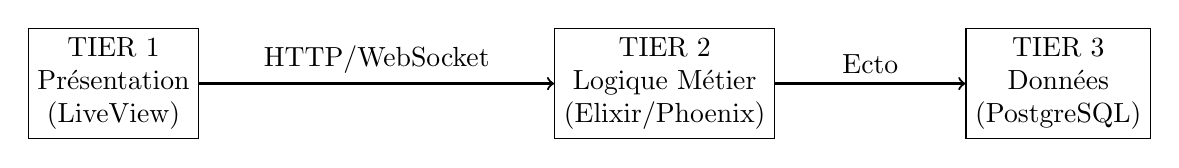
\begin{tikzpicture}[node distance=2cm]
            \node (tier1) [draw, rectangle, align=center] {TIER 1\\Présentation\\(LiveView)};
            \node (tier2) [draw, rectangle, right of=tier1, xshift=5cm, align=center] {TIER 2\\Logique Métier\\(Elixir/Phoenix)};
            \node (tier3) [draw, rectangle, right of=tier2, xshift=3cm, align=center] {TIER 3\\Données\\(PostgreSQL)};

            \draw[->, thick] (tier1) -- node[above] {HTTP/WebSocket} (tier2);
            \draw[->, thick] (tier2) -- node[above] {Ecto} (tier3);
        \end{tikzpicture}
    \end{center}
\end{for_you}

\subsection{Avantages de l'architecture 3 tiers}

\textbf{Avantages de mon architecture :} \textit{Elixir et Phoenix sont conçu pour fonctionner en archetucture 3 tiere avec des outils a disposition.\newline}

\begin{for_you}{Pourquoi ce choix ?}
    \begin{itemize}
        \item \textbf{Séparation des responsabilités} :
              Chaque tier a un rôle clair (ex. : le frontend ne gère pas la logique métier).
        \item \textbf{Scalabilité} :
              Possibilité de scaler chaque tier indépendamment (ex. : ajouter des nœuds Phoenix).
        \item \textbf{Maintenabilité} :
              Modifications isolées (ex. : changer l’UI sans toucher au backend).
        \item \textbf{Tests} :
              Tests unitaires par tier (ex. : tester les contrôleurs sans base de données).
        \item \textbf{Sécurité} :
              Contrôle d’accès par tier (ex. : le frontend n’accède pas directement à la base).
        \item \textbf{Performance} :
              Optimisation ciblée (ex. : index PostgreSQL pour les requêtes lentes).
    \end{itemize}
\end{for_you}

\section{Développement Frontend}

\begin{for_you}{Mon approche frontend avec LiveView}
    \textbf{Pourquoi LiveView ?}
    \begin{itemize}
        \item \textbf{Interactions en temps réel} :
              Mises à jour instantanées sans JavaScript côté client.
        \item \textbf{Sécurité renforcée} :
              Le traitement des données reste sur le serveur (pas de code sensible côté client).
        \item \textbf{Optimisé pour Elixir} :
              Intégration native avec Phoenix (pas besoin de framework JS externe).
    \end{itemize}

    \textbf{Structure du frontend} :
    \begin{verbatim}
    lib/badge_reader_web/
    +-- components/      # Composants réutilisables (ex: badge_card.ex)
    +-- controllers/      # Contrôleurs LiveView
    +-- views/            # Templates HTML/HEEx
    +-- router.ex         # Routes
    +-- endpoint.ex       # Configuration du endpoint HTTP
    \end{verbatim}

    \textit{Exemple de composant accessible} :
    \begin{lstlisting}
    # lib/badge_reader_web/components/core_components.ex
    def button(%{rest: rest} = assigns) do
        variants = %{"primary" => "btn-primary", nil => "btn-primary btn-soft"}

        assigns =
        assign_new(assigns, :class, fn ->
            ["btn", Map.fetch!(variants, assigns[:variant])]
        end)

        if rest[:href] || rest[:navigate] || rest[:patch] do
        ~H"""
        <.link class={@class} {@rest}>
            {render_slot(@inner_block)}
        </.link>
        """
        else
        ~H"""
        <button class={@class} {@rest}>
            {render_slot(@inner_block)}
        </button>
        """
        end
    end
    \end{lstlisting}
\end{for_you}

\begin{for_you}{Accessibilité et UX}
    \textbf{Accessibilité et UX} :
    \begin{itemize}
        \item Respect des standards \textbf{RGAA/WCAG} (ex. : balises \texttt{aria-*}).
        \item Audit avec \textbf{Lighthouse} pour mesurer :
              \begin{itemize}
                  \item Performance (FCP, LCP).
                  \item Accessibilité (contraste, labels).
              \end{itemize}
    \end{itemize}

    \textit{Exemple de rapport Lighthouse} :
    \begin{lstlisting}[language=json]
    {
      "categories": {
        "performance": {"score": 0.92},
        "accessibility": {"score": 0.98},
        "best-practices": {"score": 0.95}
      },
      "audits": {
        "first-contentful-paint": {"score": 0.95},
        "color-contrast": {"score": 1.0}
      }
    }
    \end{lstlisting}
\end{for_you}

\section{Développement Backend}

\begin{for_you}{Structure backend :}
    \begin{verbatim}
    lib/badge_reader/
    +-- application.ex    # Superviseur d'application
    +-- mailer.ex         # Emails transactionnels
    +-- repo.ex            # Configuration Ecto
    +-- contexts/          # Logique métier par domaine
    |   +-- projects/      # Gestion des projets
    |   +-- users/         # Gestion des utilisateurs
    \end{verbatim}

    \textbf{Exemple de contrôleur avec validation} :
    \begin{lstlisting}
    # lib/badge_reader/user.ex
        
        ...
        def creat_user(new_user, params) do
            changeset(new_user, params)
            new_user = params
            BadgeReader.Repo.insert(new_user)
        end

        def changeset(user, params \\ %{}) do
            user
            |> Ecto.Changeset.cast(params, [:id, :first_name, :last_name, :email, :password])
            |> Ecto.Changeset.validate_required([:first_name, :last_name, :email, :password])
        end
    end
    \end{lstlisting}

    \textit{Bonnes pratiques} :
    \begin{itemize}
        \item \textbf{Validation des données} :
              Utilisation de \textbf{Ecto.Changeset} pour valider les entrées.
    \end{itemize}
\end{for_you}

\section{Liens utiles}

\begin{itemize}
    \item Phoenix Framework : \url{https://www.phoenixframework.org/}
    \item LiveView : \url{https://hexdocs.pm/phoenix_live_view/Phoenix.LiveView.html}
    \item Ecto : \url{https://hexdocs.pm/ecto/Ecto.html}
    \item PostgreSQL : \url{https://www.postgresql.org/docs/}
    \item RGAA : \url{https://accessibilite.numerique.gouv.fr/}
    \item Lighthouse : \url{https://developers.google.com/web/tools/lighthouse}
\end{itemize}
